\chapter[AutoAdapter-Bench]{AutoAdapter-Bench: LLMs for Robot Drivers}
\label{chapter:autoadapter-bench}

\begin{quote}\itshape
The objective of this chapter is to present AutoAdapter-Bench, which separately
evaluates LLMs on driver synthesis and driver use. After setting out the
background and research questions, the chapter describes the benchmark and
experimental design. It then presents and discusses the results, concluding
with a summary that leads into the cross-robot evaluation in Chapter 5.
\end{quote}

\section[Introduction]{Introduction}

Comparing LLMs within Auto-Adapter requires distinguishing driver quality from
planning performance. When the LLM changes in both roles, differences in
end-to-end task success can arise from implementation, planning, or their
interaction.

HumanEval evaluates generated programs for functional correctness
\citep{chen2021codex}, whereas ProgPrompt evaluates task plans constructed from
supplied robot actions \citep{singh2023progprompt}. These approaches motivate
separate evaluation of the implementation behind an interface and the decisions
made through it. For driver synthesis, this requires a fixed behavioural
specification and a verdict based on independently recorded robot state.

AutoAdapter-Bench evaluates these capabilities separately in MuJoCo, using
SO-101 and Unitree Go2 as representatives of robotic arms and quadrupeds,
respectively. For each robot, the synthesis experiment measures how often each
LLM produces a driver that meets the same interface and behavioural
requirements. The driver-use experiment measures task completion while keeping
the validated driver, task conditions and planning procedure fixed within each
robot. The aim is to support model selection for each role within the evaluated
configurations.



\section[Background and Research Questions]{Background and Research Questions}

\subsection[Comparability in Driver Synthesis]{Comparability in Driver Synthesis}

Chapter 3 describes driver synthesis as an iterative process in which an LLM
implements a specified capability interface. Development simulations expose
the resulting robot state and execution errors, allowing the LLM to revise its
implementation before submitting the driver. Later driver submissions can
also incorporate diagnostic feedback from validation.

Execution feedback guides development, while independent behavioural
assessment establishes whether the resulting driver meets its requirements.
Passing individual tests provides evidence about specific capabilities but
does not establish conformance to the complete behavioural standard.

\subsection[Research Questions]{Research Questions}

AutoAdapter-Bench therefore treats observed performance as conditional on a
fixed model-plus-endpoint configuration and experimental route, rather than as
an intrinsic property of a model family. The chapter addresses two questions:

\paragraph{\textit{RQ2a---Driver synthesis.}}
With each robot's capability interface and behavioural tests held fixed,
how do the four LLM configurations differ in complete-suite validation pass rates?

\paragraph{\textit{RQ2b---Driver use.}}
When each robot's capability-validated driver and task conditions are held
constant, to what extent do the seven LLM configurations differ in
independently judged complete-task success?

The first question concerns generation of the robot-facing software layer. The
second concerns downstream use of that already fixed layer. Neither experiment
compares alternative synthesis frameworks or controller architectures.

\section[AutoAdapter-Bench]{AutoAdapter-Bench}

\noindent\textbf{Robot zoo.} AutoAdapter-Bench lists fourteen robot platforms
across seven embodiment types. The
inventory comprises seven fixed serial arms and two quadrupeds. It also
includes a dexterous hand, a humanoid, a mobile manipulator, a bimanual
manipulator and a legged mobile manipulator.

\noindent\textbf{Task suites.} AutoAdapter-Bench provides downstream task suites
in MuJoCo (Appendix~\ref{sec:appendix-tasks}). Physical outcomes are assessed
from post-step simulator state using
task-specific criteria, such as end-effector position error, object displacement
and body height.
Tool calls issued by the ReCAP high-level controller are replayed in a fresh
simulator before scoring. The learned baselines, Diffusion Policy and OpenVLA,
run directly. Onboarding assesses structural validity and remains separate
from downstream task evaluation.

\noindent\textbf{Agent models.} The benchmark includes seven LLM configurations:
Claude Sonnet 4.6, Claude Opus 5, Claude Haiku 4.5, Amazon Nova Pro,
DeepSeek V4 Pro, Ministral 3 8B and GPT-5.6 Sol. For driver use, these models
operate within ReCAP through a supplied capability interface. Exact model
identifiers and the per-token pricing used for cost estimates are listed in
Tables~\ref{tab:appendix-model-identities} and
\ref{tab:appendix-model-pricing}, respectively.

\section[Experimental Configuration]{Experimental Configuration}
\label{sec:benchmark-experiment-design}

\noindent\textbf{Driver synthesis (Experiment~2a).} Experiment~2a compared
Claude Sonnet 4.6, Claude Opus 5, Claude Haiku 4.5 and DeepSeek V4 Pro on
driver synthesis for SO-101 and Unitree Go2. For each robot, documentation
and task requirements were held constant. The capability interface and
behavioural tests remained fixed across models and independent runs.
Models generated and revised only the driver implementation. The design
specified three independent runs per model--robot combination, giving
24 scheduled trials. Each run allowed up to two revisions informed by
validation feedback. Drivers were assessed against the shared tests using
independently recorded MuJoCo state. Complete-suite pass rates, runtime and
token usage are reported.

\noindent\textbf{Driver use (Experiment~2b).} Experiment~2b compares seven LLM
configurations on task execution through supplied drivers, with five tasks per robot
(Figure~\ref{fig:chapter4-exp2b-task-scenes}).
Each robot uses a fixed, capability-validated driver and interface. The ReCAP
planning procedure and each task's initial conditions remain unchanged across
models. An independent evaluator judges task completion from MuJoCo state.
Success requires all task-specific criteria to pass. Performance is measured
by task-success rate and estimated cost per episode.

The five SO-101 tasks evaluate different forms of object manipulation.
Push to Goal requires pushing a tabletop object into a target region through
contact. Sweep into Goal uses a lateral sweeping motion to move an object
into a tabletop opening. Pick and Place requires grasping an object,
transporting it to an elevated target and releasing it. Pick and Place with
Wall adds a barrier that the grasped object must be lifted over before
placement. Dial Turn requires rotating a mounted dial to its target position
through gripper or end-effector contact.

The five Unitree Go2 tasks evaluate locomotion and obstacle traversal.
Single-step Ascent and Single-step Descent require all four feet to pass
beyond the far edge of an upward or downward step, respectively.
Mixed-obstacle Path requires crossing a ramp, raised platform, stairs and
blocks in sequence. Pause-table Transition requires moving between two
separated tables and holding position on the end table for five seconds.
Weave Poles requires following five ordered waypoints that alternate around
the poles while maintaining clearance.

\begin{figure}[htbp]
  \centering
  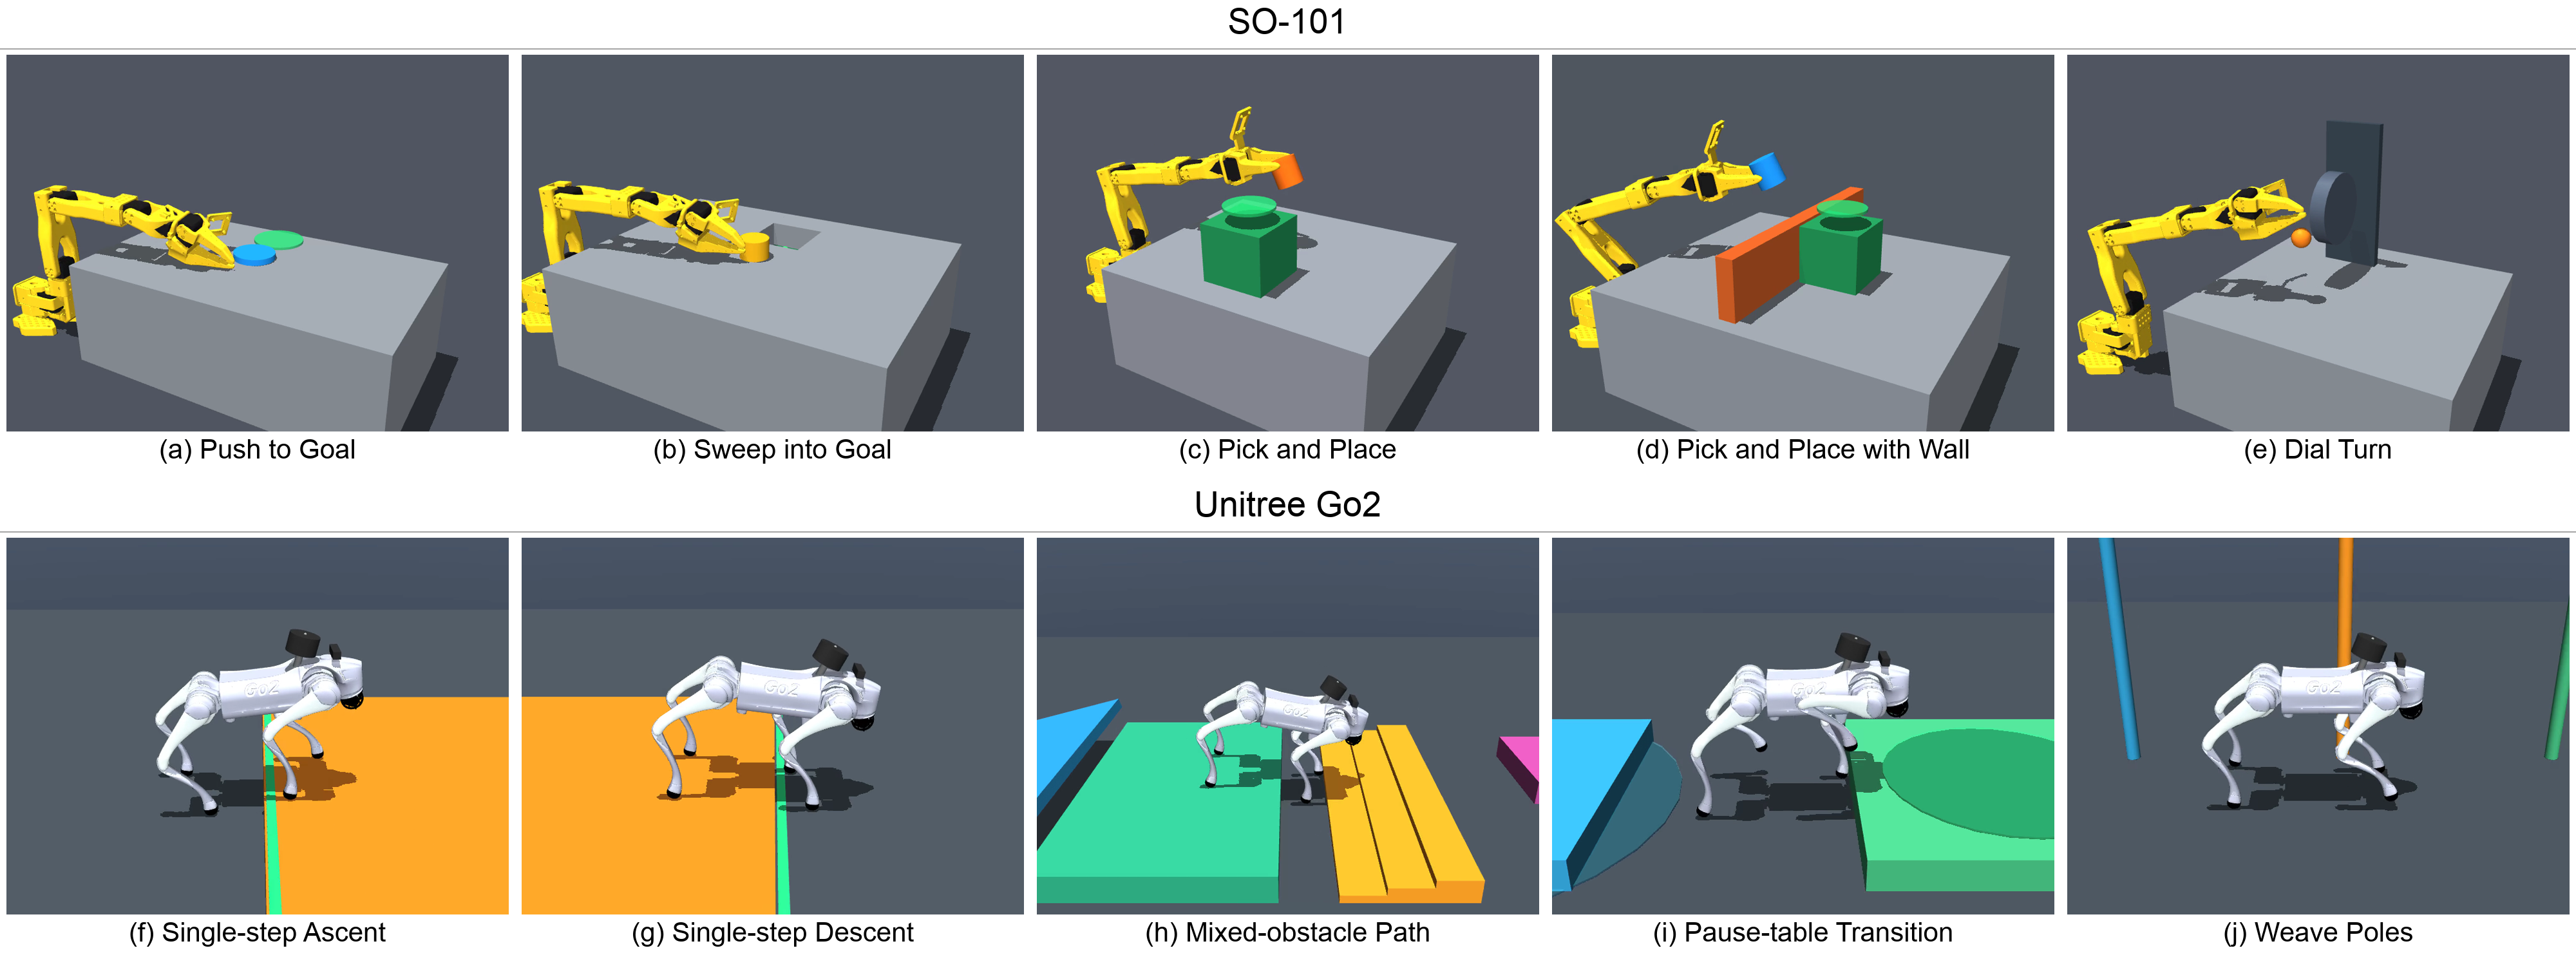
\includegraphics[width=0.95\linewidth]{assets/exp1b_task_scenes_horizontal.png}
  \caption[Corrected Experiment~2b task scenes]
  {Corrected Experiment~2b MuJoCo task scenes.
  \textbf{Top:} SO-101 Push to Goal, Sweep into Goal, Pick and Place, Pick and
  Place with Wall, and Dial Turn.
  \textbf{Bottom:} Unitree Go2 Single-step Ascent, Single-step Descent,
  Mixed-obstacle Path, Pause-table Transition, and Weave Poles.
  The panels identify evaluation conditions rather than task outcomes.}
  \label{fig:chapter4-exp2b-task-scenes}
\end{figure}

\section[Result]{Result}

\subsection[Experiment 2a: Driver Synthesis]{Experiment 2a: Driver Synthesis}
\label{sec:chapter4-exp2a-results}
\label{sec:chapter4-generation-outcomes}

\begin{table}[H]
  \centering
  \begingroup
  \small
  \setstretch{1.0}
  \setlength{\tabcolsep}{2.5pt}
  \renewcommand{\arraystretch}{1.22}
  \caption{Driver synthesis outcomes and resource use in Experiment~2a.}
  \label{tab:chapter3-exp2a-skeleton-r01-results}
  \label{tab:chapter4-exp2a-generation-results}
  \begin{tabularx}{\textwidth}{@{}>{\raggedright\arraybackslash}X
    *{2}{>{\centering\arraybackslash}p{15.9mm}
          >{\centering\arraybackslash}p{11mm}
          >{\raggedleft\arraybackslash}p{10mm}
          >{\raggedleft\arraybackslash}p{11.7mm}}@{}}
    \toprule
    \multirow{2}{*}{\textbf{LLM}} &
    \multicolumn{4}{c}{\textbf{SO-101}} &
    \multicolumn{4}{c}{\textbf{Unitree Go2}} \\
    \cmidrule(lr){2-5}\cmidrule(lr){6-9}
    & \textbf{Automatic}
    & \shortstack{\textbf{Incl.}\\\textbf{review}}
    & \shortstack{\textbf{Time}\\\textbf{(min)}}
    & \shortstack{\textbf{Tokens}\\\textbf{(k)}}
    & \textbf{Automatic}
    & \shortstack{\textbf{Incl.}\\\textbf{review}}
    & \shortstack{\textbf{Time}\\\textbf{(min)}}
    & \shortstack{\textbf{Tokens}\\\textbf{(k)}} \\
    \midrule
    Claude Sonnet 4.6
      & 1/3 & 3/3 & 9.1 & 51.2
      & 2/3 & 2/3 & 9.7 & 54.9 \\
    Claude Opus 5
      & 1/3 & 1/3 & 23.0 & 111.2
      & 2/3 & 2/3 & 37.7 & 160.8 \\
    Claude Haiku 4.5
      & 0/3 & 0/3 & 8.0 & 73.1
      & 0/3 & 0/3 & 13.8 & 115.5 \\
    DeepSeek V4 Pro
      & 1/2 & 2/2 & 13.7 & 97.0
      & 1/2 & 1/2 & 12.8 & 93.3 \\
    \bottomrule
  \end{tabularx}
  \par\smallskip
  {\footnotesize\raggedright
  \emph{Notes.} Pass counts refer to the complete behavioural test suite
  shared by all models for each robot.
  ``Incl.\ review'' includes additional passes supported by measurement
  corrections using recorded trajectories
  (Table~\ref{tab:appendix-exp2a-review}). Time and recorded output tokens are
  means across included trials, including failures. Denominators exclude
  interface interruptions.\par}
  \endgroup
\end{table}

\noindent\textbf{Generation outcomes.}
Some runs failed before a driver could undergo behavioural validation.
In one Go2 run, DeepSeek exhausted its generation budget without submitting a
driver. A Haiku Go2 submission contained a syntax error and could not be
executed.
On SO-101, Sonnet and Opus each achieved an automatic pass count of 1/3
(Table~\ref{tab:chapter4-exp2a-generation-results}).
Measurement review increased Sonnet's count to 3/3, while Opus remained at 1/3.
On Go2, both models
achieved 2/3, providing no observed pass-rate advantage for Opus.

\noindent\textbf{Revision behaviour and resource use.}\label{sec:chapter4-revision-resources}
Of the 14 runs that failed initial validation, four passed their complete
suites after repair (4/14). Two required one repair round; the other two
required two rounds. Incorrectly scoped method definitions prevented
capability calls in one DeepSeek SO-101 run. Correcting this error increased
its pass count from 0/4 to 4/4. However, a Sonnet Go2 run fell from 1/5 to 0/5
after an incomplete revised driver was submitted. A second repair subsequently
brought the pass count to 5/5.

In the selected successful runs shown in Figure~\ref{fig:chapter4-exp2a-synthesis-traces},
Sonnet required 5.6--8.4~min, compared with 13.1--14.3~min for DeepSeek.
However, DeepSeek's estimated cost was
US\$0.35--0.40, below Sonnet's US\$4.82--6.20 and Opus's US\$15.97--18.97.
The selected DeepSeek runs included an additional repair, as shown in
Figure~\ref{fig:chapter4-exp2a-synthesis-traces}.

\begin{figure}[H]
  \centering
  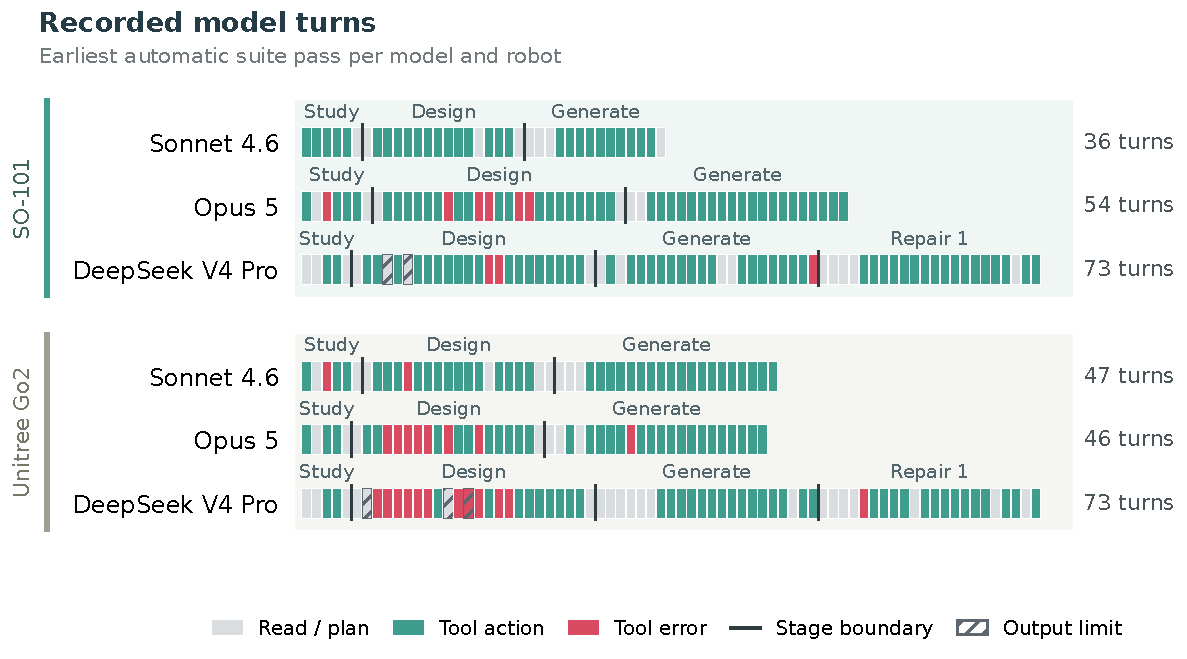
\includegraphics[width=\linewidth]{assets/exp2a_successful_run_turns.pdf}
  \caption[Model turns in selected successful synthesis runs]{Model turns in selected successful synthesis runs.}
  \label{fig:chapter4-exp2a-synthesis-traces}
\end{figure}

\subsection[Experiment 2b: Driver Use]{Experiment 2b: Driver Use}

ReCAP uses a fixed set of robot-specific driver capabilities for task
execution (Table~\ref{tab:chapter4-exp2b-driver-capabilities}).

\begin{table}[htbp]
  \centering
  \begingroup
  \small
  \setstretch{1.0}
  \renewcommand{\arraystretch}{1.12}
  \caption{ReCAP planner and robot-specific driver capabilities used in Experiment~2b.}
  \label{tab:chapter4-exp2b-driver-capabilities}
  \begin{tabularx}{\textwidth}{@{}>{\raggedright\arraybackslash}p{39mm}
    >{\raggedright\arraybackslash}X@{}}
    \toprule
    \textbf{Component / Robot} & \textbf{Configuration or Provided Capabilities} \\
    \midrule
    High-level planner & ReCAP \citep{zhang2025recap} \\
    SO-101 & \path{move_end_effector_to_position};
      \path{trace_cartesian_path}; \path{set_gripper_opening};
      \path{approach_until_contact};
      \path{move_cartesian_offset_and_return}; \path{set_wrist_roll} \\
    Unitree Go2 & \path{track_planar_twist};
      \path{move_body_relative_pose}; \path{trace_planar_path};
      \path{set_body_height}; \path{hold_stable_stance} \\
    \bottomrule
  \end{tabularx}
  \endgroup
\end{table}

Task-success rates varied across the seven ReCAP model configurations
(Table~\ref{tab:chapter3-exp2b-model-results}).

\begin{table}[htbp]
  \centering
  \begingroup
  \small
  \setstretch{1.0}
  \renewcommand{\arraystretch}{1.12}
  \caption{Performance of seven LLMs acting as the ReCAP controller across ten tasks on SO-101 and Unitree Go2, using drivers from AutoAdapter.}
  \label{tab:chapter3-exp2b-model-results}
  \begin{tabularx}{\textwidth}{@{}X
    >{\raggedleft\arraybackslash}p{43mm}
    >{\raggedleft\arraybackslash}p{45mm}@{}}
    \toprule
    \textbf{LLM} &
    \textbf{Task-success rate} &
    \textbf{Estimated cost per task (US\$)} \\
    \midrule
    Claude Opus 5       & 100.0\% & 0.585 \\
    GPT-5.6 Sol         & 87.5\%  & 0.420 \\
    Claude Sonnet 4.6   & 83.3\%  & 0.336 \\
    Claude Haiku 4.5    & 57.9\%  & 0.112 \\
    DeepSeek V4 Pro     & 44.4\%  & 0.022 \\
    Amazon Nova Pro     & 5.0\%   & 0.139 \\
    Ministral 3 8B      & 0.0\%   & 0.024 \\
    \bottomrule
  \end{tabularx}
  \par\smallskip
  {\footnotesize\raggedright
  \emph{Note.} Results combine repeated runs of the ten tasks. Success rates
  are calculated over evaluable episodes. Runs with infrastructure failures
  or incomplete evaluation evidence are excluded, so the denominator varies
  between models.\par}
  \endgroup
\end{table}

\begin{table}[htbp]
  \centering
  \small
  \renewcommand{\arraystretch}{1.12}
  \caption{Task-level success rates for SO-101 and Unitree Go2.}
  \label{tab:chapter3-exp2b-task-results}
  \begin{tabularx}{\textwidth}{@{}X r X r@{}}
    \toprule
    \textbf{SO-101 task} & \textbf{Success rate} &
    \textbf{Unitree Go2 task} & \textbf{Success rate} \\
    \midrule
    Push to Goal             & 71.4\% &
    Single-step Ascent       & 71.4\% \\
    Sweep into Goal          & 57.1\% &
    Single-step Descent      & 71.4\% \\
    Pick and Place           & 38.5\% &
    Mixed-obstacle Path      & 20.0\% \\
    Pick and Place with Wall & 11.1\% &
    Pause-table Transition   & 64.3\% \\
    Dial Turn                & 60.0\% &
    Weave Poles              & 0.0\% \\
    \bottomrule
  \end{tabularx}
\end{table}

Across all evaluable episodes, aggregate success was almost identical for SO-101 and Go2 (50.0\% and 49.2\%), placing the larger performance variation at task level (Table~\ref{tab:chapter3-exp2b-task-results}) rather than between robot platforms. Weave Poles failed in all 11 evaluable episodes because none completed the five alternating 0.12\,m waypoint regions in order (median one completed; see the example in Figure~\ref{fig:chapter3-exp2b-task-examples}(c)); nine nevertheless met the 0.10\,m torso-clearance requirement and all passed terminal stability. In all eight evaluable Pick and Place with Wall failures, the object rose by at most 7.1\,mm and moved at most 2.9\,cm from its start while contact integrity remained valid, whereas the sole success recognised an unsuccessful first grasp, issued a fully closed re-grasp, and then followed the elevated route.

Figure~\ref{fig:chapter3-exp2b-task-examples} contrasts two successful
episodes with a failed episode. Panel~(a) records GPT-5.6 Sol using SO-101
to grasp and place the object, while panel~(b) records Claude Sonnet 4.6
guiding Go2 through the Mixed-obstacle Path. Panel~(c), also from Claude
Sonnet 4.6, shows Go2 remaining clear and stable but completing only one of
five ordered waypoints.

\begin{figure}[H]
  \centering
  \begingroup
  \small
  \setstretch{1.0}
  % Keep the original frames and typeset the panel labels without run IDs.
  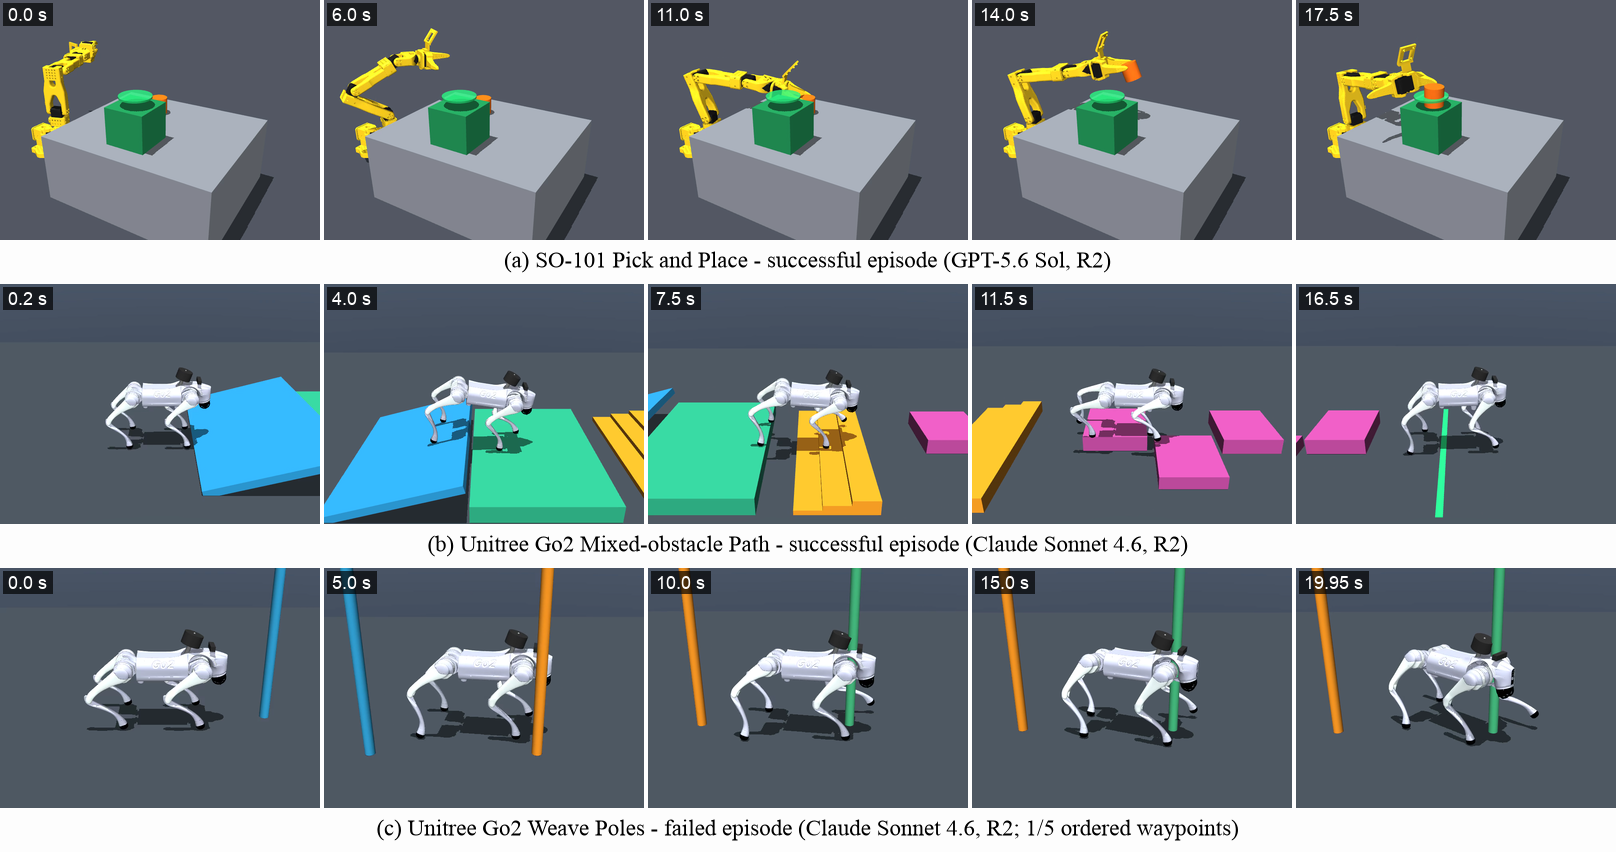
\includegraphics[width=\textwidth,trim=0 612bp 0 0,clip]{assets/exp1b_task_trajectory_examples.png}\par
  (a) SO-101 Pick and Place - successful episode (GPT-5.6 Sol)\par\smallskip
  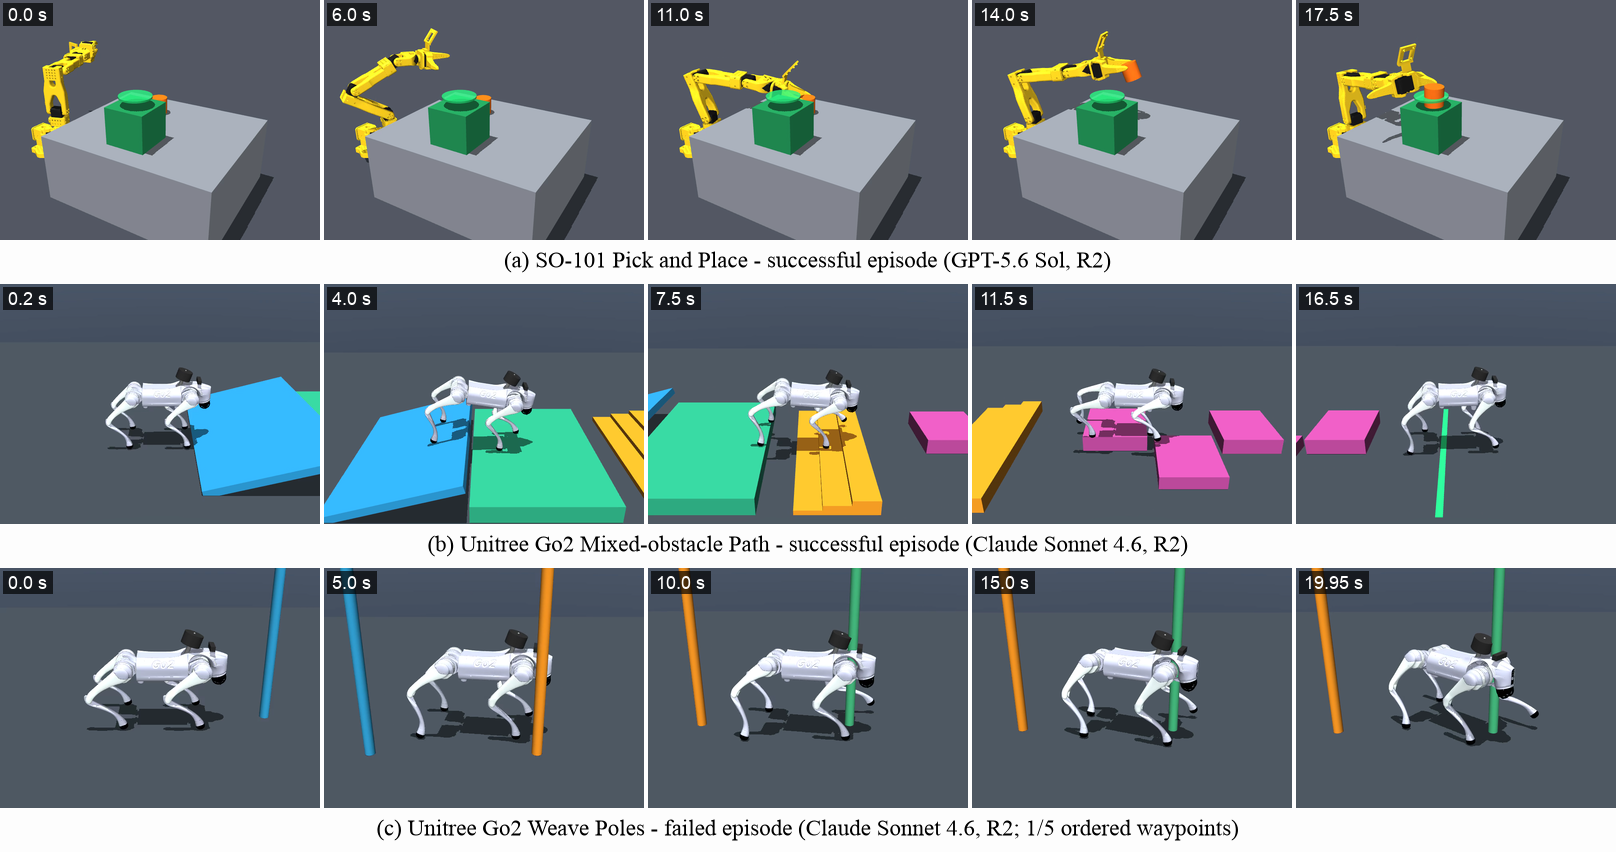
\includegraphics[width=\textwidth,trim=0 328bp 0 284bp,clip]{assets/exp1b_task_trajectory_examples.png}\par
  (b) Unitree Go2 Mixed-obstacle Path - successful episode (Claude Sonnet 4.6)\par\smallskip
  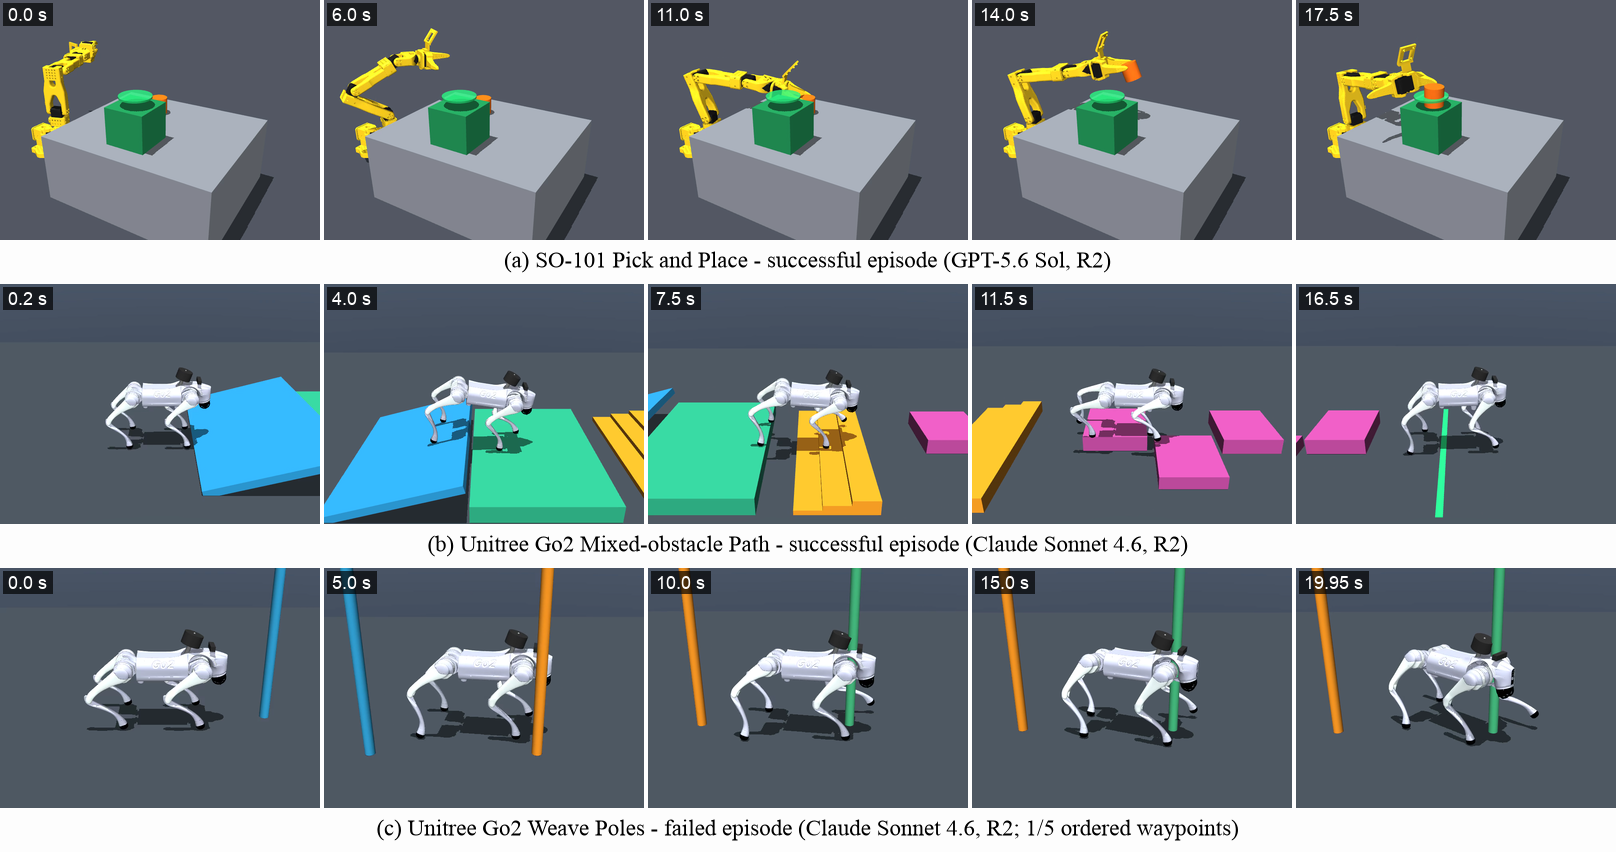
\includegraphics[width=\textwidth,trim=0 44bp 0 568bp,clip]{assets/exp1b_task_trajectory_examples.png}\par
  (c) Unitree Go2 Weave Poles - failed episode (Claude Sonnet 4.6; 1/5 ordered waypoints)\par
  \endgroup
  \caption[Experiment~2b trajectory examples]
  {Five-frame Experiment~2b trajectory examples.
  \textbf{(a)} successful SO-101 Pick and Place (GPT-5.6 Sol);
  \textbf{(b)} successful Unitree Go2 Mixed-obstacle Path
  (Claude Sonnet 4.6);
  \textbf{(c)} failed Unitree Go2 Weave Poles (Claude Sonnet 4.6).
  The failed episode passed execution, integrity, clearance, stability, and
  video checks but completed only one of five ordered waypoints.}
  \label{fig:chapter3-exp2b-task-examples}
\end{figure}

\section[Discussion]{Discussion}

Even with validated drivers, task completion may be limited by action
sequencing and failure recovery. In Weave Poles, the robot remained stable
at termination but did not complete the required waypoint sequence. The object
was barely lifted in failed Pick and Place with Wall episodes; the successful
episode included a second grasp. These trajectories suggest that high-level
controllers need to check intermediate outcomes and adjust subsequent actions.

Validation feedback helped correct some implementation errors, but successive
revisions did not consistently increase the number of tests passed. Among the
successful runs shown, Sonnet completed synthesis faster, while DeepSeek had
lower estimated costs. Repair counts alone therefore do not measure resource
efficiency; model selection should consider validation outcomes, time and cost.

Holding each robot's capability interface and behavioural tests fixed makes
driver implementation the focus of the synthesis comparison. Automatic passes
establish conformance to the shared tests under the evaluated conditions.
Measurement reviews are reported separately from the original automatic verdicts.

The findings are limited to the evaluated model configurations, robots, tasks
and MuJoCo conditions. Model rankings are provisional, and further repeated
trials are needed to assess their stability. Similar aggregate success rates
across the two robots do not establish that morphology has no effect.
Chapter 5 examines other robot configurations to assess the scope of these
observations.

\section{Summary}

This chapter introduced AutoAdapter-Bench and compared four LLM configurations
for driver synthesis and seven for driver use on SO-101 and Unitree Go2.
In driver synthesis, Sonnet matched Opus's automatic pass counts with shorter
runtimes and fewer output tokens. DeepSeek had lower estimated costs in the
successful synthesis runs shown. Validation feedback helped some initially
unsuccessful runs pass their complete test suites, although successive
revisions did not consistently improve outcomes.

With the drivers, task conditions and ReCAP planning procedure held fixed,
Opus achieved the highest complete-task success rate. Haiku did not generate
a driver that passed its complete validation suite, yet completed some tasks
using supplied drivers. Execution traces also revealed difficulties with
ordered waypoint traversal and grasp recovery. Robots could remain stable
without completing the required task sequence. These results show that
performance in using existing drivers does not directly establish a model's
driver-synthesis ability.
